\documentclass[french,12pt]{article}
\usepackage[utf8]{inputenc}
\usepackage[T1]{fontenc}
\usepackage{lmodern}
\usepackage[a4paper]{geometry}
\usepackage{babel}
\usepackage{xcolor}   
\usepackage{amsmath}
\usepackage{booktabs}
\usepackage{amsfonts}
\usepackage{amssymb}
\author{Thomas \bsc{Lantz}}
\usepackage{graphicx}
\usepackage{listings}
\usepackage{color}
\usepackage{float}
\restylefloat{table}
\usepackage{textcomp}
\usepackage{pgfplots,pgfplotstable}
\usepackage{url}
\usepackage{tikz}
\usetikzlibrary{arrows,backgrounds,mindmap,positioning,shadows,shapes}
\definecolor{listinggray}{gray}{0.9}
\definecolor{lbcolor}{rgb}{0.9,0.9,0.9}

\pgfplotstableset{
every head row/.style={before row=\toprule,after row=\midrule},
every last row/.style={after row=\bottomrule}}


\lstset{
	backgroundcolor=\color{lbcolor},
	tabsize=4,
	rulecolor=,
	language=C++,
        basicstyle=\scriptsize,
        upquote=true,
        aboveskip={0.5\baselineskip},
        columns=fixed,
        showstringspaces=false,
        extendedchars=true,
        breaklines=true,
        prebreak = \raisebox{0ex}[0ex][0ex]{\ensuremath{\hookleftarrow}},
        frame=single,
        showtabs=false,
        showspaces=false,
        showstringspaces=false,
        identifierstyle=\ttfamily,
        keywordstyle=\color[rgb]{0,0,1},
        commentstyle=\it\tt\color[rgb]{0.133,0.545,0.133},
        stringstyle=\color[rgb]{0.627,0.126,0.941},
        inputencoding=utf8
        }

\lstset{escapeinside={(*@}{@*)}}
\lstset{includerangemarker=false,rangeprefix=\/\/\#\ ,% curly left brace plus space
  rangesuffix=\ \#}% space plus curly right brace



\begin{document}
\begin{titlepage}
\begin{center}
  \Huge
  \textbf{UFR de Mathématiques et d'Informatique de Strasbourg}
  \par \vspace{2 cm}
  \textbf{Rapport de Stage}
  \par \vspace{1 cm}
  \emph{Wrapping Python}
  \par \vspace{5 cm}
  \bsc{Lantz} Thomas
  \par \vspace{3 cm}
  \normalsize{\today}\\
  \end{center}
\end{titlepage}

\newpage
\tableofcontents
\newpage

\section{Introduction et présentation des outils}

Afin de débuter ce rapport,commençons par énoncer le sujet sur lequel j'ai travaillé et présenter par la même occasion certains des différents outils qui seront utilisé au cours de celui-ci.

\subsection{Introduction au sujet}

La compilation d'un fichier en C++ est nécessaire à chaque modification de celui-ci et elle est d'autant plus longue que son contenu est grand, notamment en y ajoutant des éléments de la librairie Feel++. Alors quand il est question de ne modifier qu'un paramètre,la dimension des éléments du maillage par exemple, pour divers tests, le fait de devoir recompiler à chaque changement peut nous faire perdre pas mal de temps.
\newline

Le sujet de mon stage, le Wrapping Python du code Feel++, a pour but d'essayer de corriger cela.En effet, le wrapping consiste à récupérer des classes et méthodes déjà implémentées ( ici en Feel++/C++) afin de pouvoir créer un module Python qui nous permettra les utiliser dans un nouveau langage(ici Python) grâce à des outils divers que l'on présentera après.
\newline

Le Python étant un langue non compilé mais interprété, la modification dans le script d'un paramètre n'entraînera pas de recompilation et l'exécution se fera de suite après cela.
\newline

Ainsi il nous suffira donc de construire le module Python à partir des outils et codes déjà implémentés, de compiler celui-ci une seule fois, et l'on pourra alors utiliser toutes les méthodes et classes ainsi récupérées dans un script Python.
\newline

Après avoir présenté certains outils qui seront utilisés lors de ce stage,on pourra alors commencer la présentation du travail effectué lors de ces 2 mois,en essayant de part ce fait vous expliquer le fonctionnement et l'utilisation du wrapping Python.

\subsection{Outils utilisés}

\subsubsection{Trello}

Trello est une plateforme d'organisation de travail en ligne.Elle est organisée sous forme de board(ou tableau) dont on définit l'accès aux différents participants.
\newline

Chaque board peut-être décomposé en sous-sections que l'on créera et qui contiendra des cartes définissant les différentes tâches voulues.
Chaque carte, outre son titre, peut être complétée avec toutes sortes d'informations comme des liens, des images ou des paliers à accomplir pour la réalisation d'une tâche et peut être limité à modification par les participants voulues.
\newline

De même, ces cartes peuvent à tout moment être déplacées entre les différentes sections du board, ce qui permet par exemple de voir dans notre cas le travail à faire,celui qui est en cours et ceux qui sont finis.
\newline

Voici par exemple une capture d'écran d'un de mes boards associé au stage durant celui ci :

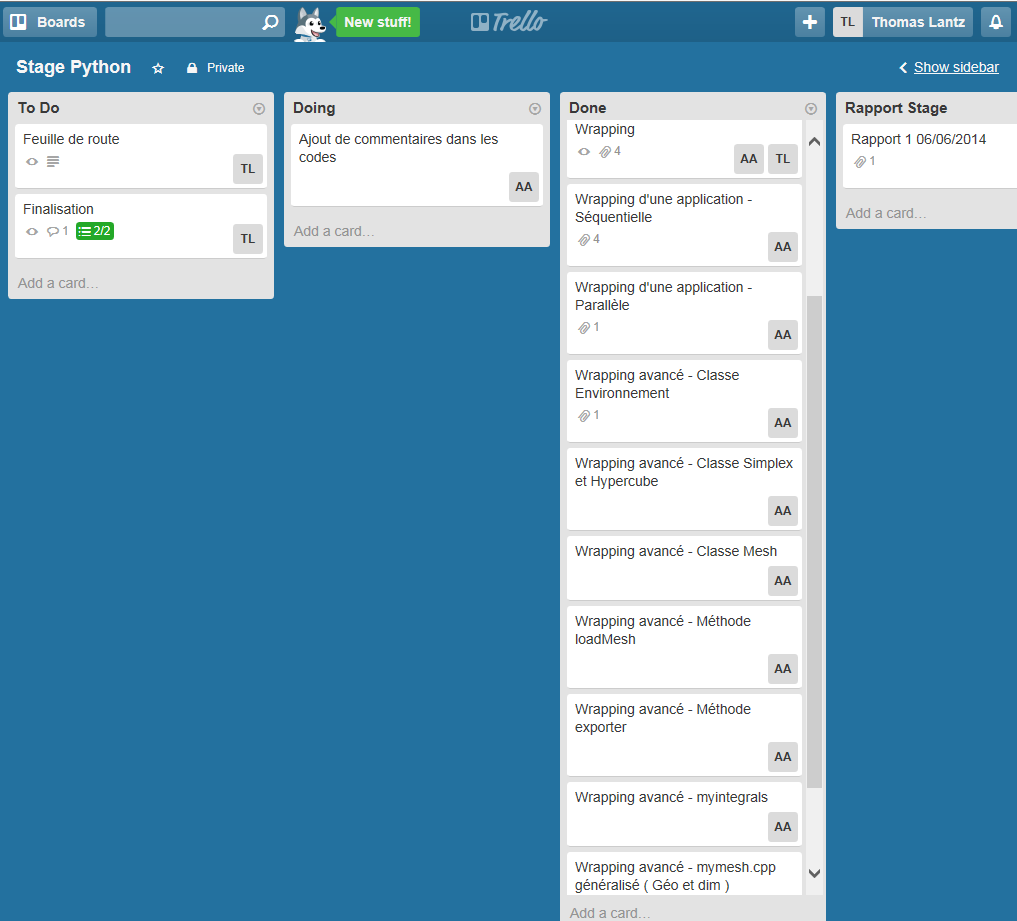
\includegraphics[scale=0.60]{1.png} 

\subsubsection{Github/Git}

Github est, quand à lui, une plateforme de stockage de projets en ligne.On crée, ou rejoint, un projet et on peut alors y stocké toutes sortes de documents, qui ne pourront être modifié directement uniquement par les participants autorisés.
Pour les autres, il est possible de récupérer une copie du projet, afin de travailler dessus et ensuite soumettre son travail qui pourra alors être intégré o u non au projet selon les résultats fournis.
\newline

L'un des gros avantages de Github est, qu'en plus de fournir un accès entièrement par terminal avec des commandes associées ( commençant par git .....), est qu'il conserve une trace de toutes les modifications d'un fichiers qui ont été effectuées.Cela permet de récupérer une fichier suite à une modification qui semblait au premier abord, mais cause des soucis avec d'autres fichiers par exemple.
   
\subsubsection{Vim}

Qui dit code à écrire, dit éditeur de texte....et sur la plateforme atlas sur laquelle on travaille, l'éditeur présent est Vim. Vim est donc un éditeur de texte associé au terminal, et permet alors d'ouvrir des fichiers directement dans celui-ci.La prise en main n'est pas forcément évidente au début, mais une fois que l'on s'y est fait et que l'on connaît quelques raccourcis, on remarque alors que Vim est un éditeur de texte très puissant.

\subsubsection{Cmake}

CMake ( ou cross plateform make) est, comme son nom l'indique, un programme de construction multi-plateforme.Son usage ressemble beaucoup à la commande make, mais Cmake est une version plus avancé de celle-ci.
\newline

Grâce à des fichiers de configuration, appelé CMakelists.txt, il permet de gérer et générer toutes sortes de fichiers, par exemple créer les exécutables associés à chaque fichier codé en Feelpp voulu, ou même lié des librairies déjà existantes à des nouveaux programmes pour en récupérer les données nécessaires à la compilation.

\newpage
\section{Wrapping Python}
Après cette rapide présentation du sujet et des outils,nous allons pouvoir entrer dans le vif du sujet, en explicitant dans cette partie, le travail effectué pendant ces 2 mois et introduire de cette façon le manière dont j'ai procédé pour créer une librairie Python, ainsi que les difficultés que j'ai pu rencontré à chaque étape.

Tous les exemples traités sont présents intégralement 
\subsection{Boost.Python}
Commençons par introduire certainement l'outil le plus important de ce stage qui nous permettra de mettre en place les différentes librairies Python à partir du code Feel++ : Boost.Python.
\newline

Boost.Python est une librairie C++ qui permet de transposer du code entre le C++ et Python. Elle permet en effet de récupérer des classes et méthodes déjà présentes en C++ afin de définir directement, à partir de leur définition, un équivalent en Python. 
\newline

Pour se faire, on utilisera alors la syntaxe suivante que l'on placera dans un fichier qu'on compilera afin de créer la bibliothèque :

\begin{lstlisting}
#include <boost/python.hpp>
#include <mpi4py/mpi4py.h>

BOOST_PYTHON_MODULE("libName")
{
 if (import_mpi4py()<0) return ;
 .....
 .....
}

\end{lstlisting}

avec "Name" le nom de la librairie voulue que l'on fera précédé d'un préfixe lib et à l'intérieur des accolades les classes et méthodes que l'on veut importer dans notre libraire Python avec une syntaxe que je présenterai plus en détail pour chaque type d'objet. On utilise également la méthode import\_mpi4py()afin de vérifier que MPI est bien initialisé dans le script Python à partir du module mpi4py.
\newline

Il ne nous reste plus alors qu'à donner l'information à CMake qu'il doit compiler ce fichier en créant une librairie Python. Il suffit pour cela d'adopter le code suivant :

\newpage
\begin{lstlisting}
if(FEELPP_ENABLE_PYTHON)

add_library(Name SHARED fichier.cpp)
target_link_libraries(Name feelpp ${FEELPP_LIBRARIES})

endif()
\end{lstlisting}

On pourra remarquer qu'ici on utilise uniquement le nom de la librairie sans le préfixe lib devant, ainsi que l'utilisation d'une option nommé FEEL\_ENABLE\_PYTHON rajouté dans FindFeelpp. afin de gérer si l'on veut ou non compiler ce fichier. 
\newline

On a alors créer la librairie associée aux méthodes et classes placées dans le BOOST\_PYTHON\_MODULE et il nous suffit donc de l'appeler comme n'importe quel autre module dans un script Python , comme suivant :

\begin{lstlisting}
#!/usr/bin/python

from mpi4py import MPI
import libName

t=libName.testFunction()
\end{lstlisting}

\subsection{Classes}
Commençons par voir comment wrapper les différents type de classes possibles.
Le wrapping de classe est utilisé principalement pour 2 raisons:\\
- Création d'un objet du type de la classe wrappé et utilisation des méthodes associées \\
- Récupération et définition d'un type de retour non connu par Python\\

La syntaxe de base est la suivante:
\begin{lstlisting}
class_<"info sur la classe">("Name",init);
\end{lstlisting}
avec entre crochet les différentes informations sur la classe et notamment le type que l'on veut récupérer, Name qui correspond au nom qu'auront les objets de ce type en Python et init si l'on veut y ajouter un constructeur.

\subsubsection{Wrapping de classes simples}
Les classes simples sont les classes qui ne possèdent pas de template lors de leurs définitions.Prenons comme exemple la classe Environment, dont l'un constructeur est systématiquement utilisé à chaque début de programme, et qui est défini de la sorte :

\newpage
\begin{lstlisting}
namespace Feel 
{
namespace detail
{
class Environment : boost::noncopyable
{
 ...
}
}
}
\end{lstlisting}
On veut donc pouvoir récupérer cette classe ainsi que son constructeur afin de pouvoir l'utiliser dans nos script Python. 
\newline

Pour cela, il suffit d'utiliser la syntaxe suivante :
\begin{lstlisting}
class_<Feel::detail::Environment,boost::noncopyable>("Environment",no_init);
\end{lstlisting}

On donne ainsi:\\
- la classe à wrapper, ici Feel$::$detail$::$Environment \\
- boost$::$noncopyable par définiton de Environment \\
- le nom associé à l'objet Python , ici Environment \\
- un constructeur, ici on décide de ne pas en mettre de suite. Ce sera en effet le sujet d'une autre partie.

\subsubsection{Wrapping de classes avec templates}

Les classes avec templates causent elle un peu plus de soucis pour le wrapping.
En effet, le Python étant un langage interprété et non compilé, l'utilisation de template est impossible et il faut donc remplir à chaque wrapping d'une classe les templates avec des valeurs particulières. Cela créer une barrière nous empêchant alors de transmettre du code générique au nouveau module Python.
\newline

Afin d'illustrer mes propos, prenons la classe Mesh qui s'occupe de générer les maillages et qui est défini de la sorte :
\begin{lstlisting}
template<typename GeoShape, typename T=double, int Tag=0>
class Mesh
{
 ...
}
\end{lstlisting}

On voit bien que Mesh nécessite un type d'éléments du maillages en tant que templates,et l'on ne peut pas simplement écrire :

\newpage
\begin{lstlisting}
class_<Feel::Mesh<GeoShape>,boost::noncopyable>("Mesh",init<>())
\end{lstlisting}

Il faut donc choisir un type, ici soit Simplex, soit Hypercube. Malheureusement, ces 2 types sont également liés à des templates par rapport à leurs dimensions.On doit de même définir les valeurs de ces dimensions si l'on veut récupérer un type d'objet en Python.
\newline

Ainsi pour avoir un maillage composé de triangles ( Simplex de dimension 2), il faut écrire :
\begin{lstlisting}
class_<Feel::Mesh<Feel::Simplex<2>>,boost::noncopyable>("Mesh",init<>())
\end{lstlisting}

De même, si l'on veut un maillage composé de cubes (Hypercube de dimension 3), cela nous donne :
\begin{lstlisting}
class_<Feel::Mesh<Feel::Hypercube<3>>,boost::noncopyable>("Mesh",init<>())
\end{lstlisting}

On peut déjà entrevoir ici un des problèmes du wrapping Python, avec l'obligation de définir tous les templates avec des valeurs, qui de plus s'accentuera encore un peu quand il faudra appliquer des méthodes sur des objets templatés mais ce sera le sujet d'une partie suivante.On essayera également de corriger au mieux ce problème un peu plus loin.

\subsection{Méthodes}

Après ce bref aperçu sur le wrapping de classe, passons à celui de méthodes.On retrouve ici plus de cas différents que pour les classes, mais la syntaxe est la même pour toute.
\newline
Si la méthode appartient à une classe A par exemple, on a alors :
\begin{lstlisting}
class_<A>("A",no_init)
.def("exe",A::exe);
\end{lstlisting}

Sinon on a la syntaxe suivante:
\begin{lstlisting}
def("exe",exe);
\end{lstlisting}

avec comme premier argument la nom que prendra la définition de notre méthode en Python, suivi ensuite de l'emplacement de cette méthode dans notre code Feel++.
\newline
Si une méthode rentre dans plusieurs catégories, il suffit d'appliquer les différentes méthodes ensemble pour obtenir le résultat escompté.
\subsubsection{Wrapping de méthodes simples}

Commençons par le cas le plus simple : les méthodes simples.Ce sont les méthodes sans templates présents ni dans les arguments ni dans le type de retour.
Pour ses méthodes là, il suffit d'appliquer la méthode présenté plus haut.
Par exemple, avec la méthode printMa1 définit par :
\begin{lstlisting}
void printMa1(integrate_return_type::value_type m)
{
 	std::cout << m << std::endl;
}
\end{lstlisting}

Il nous suffit alors d'écrire:
\begin{lstlisting}
def("printSol",,printMa1);
\end{lstlisting}

De même avec la méthode worldComm dans la classe Environment présentée avant,on a alors :
\begin{lstlisting}
class_<Feel::detail::Environment,boost::noncopyable>("Environment",no_init)
	.def("worldComm",&Feel::detail::Environment::worldComm,return_value_policy<copy_non_const_reference>())
	.staticmethod("worldComm");
\end{lstlisting}

Il ne faut pas oublier de wrapper un objet du type de retour, si ce n'est pas un type simple (int,char,....) ou un type appartenant à Python(boost$::$python$::$list,..).
On peut également observé ici deux nouvelles commandes:\\
- return\_value\_policy<T> qui permet d'indiquer à Python ce que la méthode doit renvoyer (ici une référence sur un objet WorldComm).\\
- staticmethod qui indique à Python que la méthode est définie statiquement.\\

Pour l'exemple précédent,par exemple, il faut lui indiquer à quoi correspond le type d'objet WorldComm de la façon suivante:
\begin{lstlisting}
class_<WorldComm>("WorldComm,init<>());
\end{lstlisting} 

Bien que ce soit le cas le plus simple,on peut déjà commencer à y rencontrer une petite difficulté, qui sera également présente dans tous les autres cas, de par la présence de pointeur dans les méthodes.\\
En effet, en Python la notion de pointeur n'est pas présente naturellement comme en C++, et quand on doit donner un $char**$ à une méthode wrappé, ce n'est pas directement possible.\\

Pour contrer ce problème, il y a deux solutions suivants le cas rencontré :\\

- Pointeur sur un type de base : Dans ce cas, on va écrire une méthode, qui à partir d'une liste Python, va créer un $char**$, appellera la méthode voulue avec , puis libérera la mémoire utilisée. C'est cette méthode qu'on wrappera alors en Python et qu'on utilisera à la place de l'autre.\\
Par exemple pour l'appel d'une méthode main comme suivant :
\begin{lstlisting}
int main(int argc,char** argv)
\end{lstlisting}

On écrit une méthode comme suivant :
\begin{lstlisting}
void wrap(boost::python::list argv)
{
	int argc=boost::python::len(argv);
	char** pyarg=new cahr* [argc+1];
	boost::python::stl_imput_iterator<std::string> gegin(argv), end;
	int i=0;	
	while(begin != end)
	{
		pyarg[i]=strdup((*begin).c_str());
		begin++;
		i++;
	}
	pyarg[argc]=NULL;
	main(argc,pyarg);
	for(int i=0;i<argc;i++)
		delete pyarg[i];
	delete[] pyarg;
}	
\end{lstlisting}

Il ne reste alors plus qu'à la wrapper:
\begin{lstlisting}
def("main",main);
\end{lstlisting}

- Pointeur sur une classe : Ici,on va travailler sur les wrapping de classes.En effet, si l'on veut appeler une méthode avec comme argument un pointeur sur un objet de type A, il y a de fortes chances que l'on ai déjà wrapper la classe A.
Il suffit alors d'ajouter après avoir donné le type, que cet objet peut également exister en temps que pointeur avec boost$::$shared\_ptr , de la sorte :
\begin{lstlisting}
class_<A,boost::shared_ptr<A>>("A",no_init)
\end{lstlisting}

\subsubsection{Wrapping de méthodes avec paramètres par défaut}

Les méthodes possédant des arguments par défaut se comporte exactement comme les méthodes associées sans arguments par défaut au niveau du wrapping.Cependant, si on se contente de les wrapper telles quelles, Python va perdre la valeur des arguments par défaut, et on ne pourra alors plus appeler celles-ci simplement avec les arguments non définis.\\
On va pour corriger cela devoir redéfinir des sous-méthodes qui seront wrappées à la place de la méthode principale: \\
Afin d’illustrer cela, prenons la méthode suivante comme exemple :

\newpage
\begin{lstlisting}
template<typename MeshType>
boost::tuple<mpl::size_t<MESH_ELEMENTS>,
	typename MeshTraits<MeshType>::location_element_const_iterator,
	typename MeshTraits<MeshType>::location_element_const_iterator>
boundaryelements(MeshType const& mesh,uint16_type entity_min_dim=0,uint16_type entity_max_dim=2)
{
 ...
}
\end{lstlisting}

On peut alors définir une méthode de la sorte qui va l'appeler, comme suivant:
\begin{lstlisting}
template<typename MeshType>
boost::tuple<mpl::size_t<MESH_ELEMENTS>,
	typename MeshTraits<MeshType>::location_element_const_iterator,
	typename MeshTraits<MeshType>::location_element_const_iterator>
boundaryelements_w(MeshType const& mesh)
{
 	return boundaryelements(mesh);
}
\end{lstlisting}

On obtient alors une méthode sans avoir d'arguments par défaut, il suffit alors de la wrapper de la même façon qu'une méthode de la sorte.

\subsubsection{Wrapping de méthodes avec templates}

Avec les méthodes possédant des templates, on va se retrouver avec le même soucis qu'avec les classes templatées, c'est à dire qu'on va devoir définir des valeurs pour chaque template. Et cela va à nouveau nous causer pas mal de soucis.\\

En effet, si un argument utilise un objet du template, la méthode ne pourra être appeler qu'avec le choix que l'on aura fait lors du remplissage de celui-ci.\\

Prenons la méthode loadMesh définie de la sorte (on expliquera dans le partie suivante comment on en est arrivé là):
\begin{lstlisting}
boost::shared_ptr<Mesh<Simplex<2>>> loadMesh_w (Mesh<Simplex<2>>* mesh)
{
 return loadMesh(_mesh=mesh);
}
\end{lstlisting}

Si l'on wrappe la méthode telle quelle est actuellement, on ne pourra l'utiliser que pour des objets du type Mesh<Simplex<2>> ce qui ne représente qu'une petite partie des types possibles que l'on pourrait avoir ici.\\

Afin de wrapper de telles méthodes,il y a deux solutions :\\

On peut soit redéfinir comme précédemment une nouvelle méthode avec les champs du template remplacé par les valeurs voulues, et l'on se retrouve avec une méthode qui ne possède plus de template.Il ne reste alors qu'à la wrapper comme présenter plus haut.\\

Ou alors on peut directement définir les valeurs voulues pour les membres du templates lors de la définition de la fonction dans le BOOST\_PYTHON\_MODULE de la façon suivante :
\begin{lstlisting}
def("Test",test<3,double>);
\end{lstlisting}

On a parlé pour l'instant uniquement des soucis avec des arguments de la méthode liés au template, mais le type de retour peut également nous amener son lot de problèmes.

En effet, comme on doit indiquer à Python le type de retour en définissant une classe dans la librairie, on ne peut pas le faire de manière générique en conservant les templates. Il faut également donner des valeurs aux différents templates lors de ces définitions,et cela peut poser problème lorsque les types deviennent assez long et compliqué à modifier pour d'autres valeurs du template.\\
Voici par exemple le type de retour du constructeur de Pch :
\begin{lstlisting}
Feel::FunctionSpace<Mesh<Simplex<2>>,Feel::bases<Feel::Lagrange<1,Feel::Scalar,Feel::Continuous,Feel::PointSetEquiSpaced,0>>,double,Feel::Periodicity<Feel::NoPeriodicity>,Feel::mortars<Feel::NoMortar>>
\end{lstlisting}

On essayera dans la dernière partie de ce rapport de trouver une solution à ce problème grâce à certains outils et librairies existantes.

\subsubsection{Wrapping de BOOST\_PARAMETER\_FUNCTION}

L'utilisation de la macro BOOST\_PARAMETER\_FUNCTION permet de générer une méthode spécifique à partir du nom, du type de retour et des arguments donnés.En effet, pour appeler une méthode crée ainsi, il faut nommer les champs d'arguments à remplir suivi de la valeur que l'on veut associer.\\
Voici un exemple d'une BOOST\_PARAMETER\_FUNCTION que l'on vu juste avant : la méthode loadMesh.

\begin{lstlisting}
BOOST_PARAMETER_FUNCTION(
    ( typename Feel::detail::mesh<Args>::ptrtype ), // return type
    loadMesh,    // 2. function name
    tag,           // 3. namespace of tag types
    ( required
      ( mesh, *)
        ) // 4. one required parameter, and
    ( optional
      ( filename, *( boost::is_convertible<mpl::_,std::string> ), option(_name="gmsh.filename").template as<std::string>() )
      ( desc, *,boost::shared_ptr<gmsh_type>() )  // geo() can't be used here as default !!
      ( h,              *( boost::is_arithmetic<mpl::_> ), option(_name="gmsh.hsize").template as<double>() )
      ( straighten,          (bool), option(_name="gmsh.straighten").template as<bool>() )
      ( refine,          *( boost::is_integral<mpl::_> ), option(_name="gmsh.refine").template as<int>() )
      ( update,          *( boost::is_integral<mpl::_> ), MESH_CHECK|MESH_UPDATE_FACES|MESH_UPDATE_EDGES )
      ( physical_are_elementary_regions,		   (bool), option(_name="gmsh.physical_are_elementary_regions").template as<bool>() )
      ( worldcomm,       (WorldComm), Environment::worldComm() )
      ( force_rebuild,   *( boost::is_integral<mpl::_> ), option(_name="gmsh.rebuild").template as<bool>() )
      ( respect_partition,	(bool), option(_name="gmsh.respect_partition").template as<bool>() )
      ( rebuild_partitions,	(bool), option(_name="gmsh.partition").template as<bool>() )
      ( rebuild_partitions_filename, *( boost::is_convertible<mpl::_,std::string> )	, filename )
      ( partitions,      *( boost::is_integral<mpl::_> ), worldcomm.globalSize() )
      ( partitioner,     *( boost::is_integral<mpl::_> ), option(_name="gmsh.partitioner").template as<int>() )
      ( partition_file,   *( boost::is_integral<mpl::_> ), 0 )
      ( depends, *( boost::is_convertible<mpl::_,std::string> ), option(_name="gmsh.depends").template as<std::string>() )
        )
    )
\end{lstlisting}
On peut alors l'appeler par exemple de la façon suivante:
\begin{lstlisting}
auto mesh = loadMesh( _mesh=new Mesh<Simplex<2>> );
\end{lstlisting}

Afin de wrapper des méthodes de ce type, il existe des méthodes spécifiques présentées dans le lien suivant :\\
\url{http://www.boost.org/doc/libs/1_46_0/libs/parameter/doc/html/python.html}
\vspace{0.5 cm}

Malheureusement je n'ai pas réussi à les appliquer et les mettre en œuvre au cours de mon stage.Je me suis alors rabattu sur une technique, voir plutôt une astuce, similaire à ce que j'ai utilisé jusqu'à présent.
Pour cela, il suffit de créer une nouvelle méthode avec le même type de retour et les arguments que l'on veut utiliser, et simplement d'appeler la fonction défini par la BOOST\_PARAMETER\_FUNCTION.\\
En reprenant l'exemple précédent de loadMesh, on obtient :
\begin{lstlisting}
boost::shared_ptr<Mesh<Simplex<2>>> loadMesh_w (Mesh<Simplex<2>>* mesh)
{
 return loadMesh(_mesh=mesh);
}
\end{lstlisting}

Il suffit alors comme plus haut de wrapper cette nouvelle fonction et de l'utiliser dans notre script Python.Cependant,de part cette astuce, on perd la possibilité de pouvoir appeler la méthode originelle avec les champs et arguments voulus, modifiable à tout moment dans le script Python.

\subsection{Trucs et Astuces}
On va, dans cette section, rapidement présenté quelques astuces facilitant le wrapping de classes et méthodes.
\subsubsection{Récupération du type de retour}
Wrapper le type de retour peut être particulièrement difficile, notamment quand il est remplacé par un typename dans la définition de la méthode et , quand plus de cela, il est composé de template. On doit alors donner le type exact de retour avec les templates remplis pour pouvoir utiliser un objet de ce type.\\

C'est la qu'intervient une astuce,nommé "give bad to have good", dont l'idée m'est venu suite à une discution sur le type de retour de la méthode integrate avec mes camarades de stage.En effet, suite à cela, l'un d'entre eux a exposé la théorie suivante : " De toute façon, une intégrale ça renvoie un double, non ?".\\

L'idée est donc de donner un type de base que l'on sait faux de toute façon, et attendre alors que la compilation nous renvoie alors l'erreur avec le type à récupérer. J'ai ainsi pu récupérer notamment des types comme le suivant qui serait en temps normal introuvable aussi rapidement:

\begin{lstlisting}
typedef boost::tuples::tuple<mpl_::size_t<0ul>, boost::multi_index::detail::bidir_node_iterator<boost::multi_index::detail::ordered_index_node<boost::multi_index::detail::ordered_index_node<boost::multi_index::detail::ordered_index_node<boost::multi_index::detail::ordered_index_node<boost::multi_index::detail::ordered_index_node<boost::multi_index::detail::ordered_index_node<boost::multi_index::detail::ordered_index_node<boost::multi_index::detail::index_node_base<Feel::GeoElement3D<(unsigned short)3, Feel::Simplex<(unsigned short)3, (unsigned short)1, (unsigned short)3>, double>, std::allocator<Feel::GeoElement3D<(unsigned short)3, Feel::Simplex<(unsigned short)3, (unsigned short)1, (unsigned short)3>, double> > > > > > > > > > >, boost::multi_index::detail::bidir_node_iterator<boost::multi_index::detail::ordered_index_node<boost::multi_index::detail::ordered_index_node<boost::multi_index::detail::ordered_index_node<boost::multi_index::detail::ordered_index_node<boost::multi_index::detail::ordered_index_node<boost::multi_index::detail::ordered_index_node<boost::multi_index::detail::ordered_index_node<boost::multi_index::detail::index_node_base<Feel::GeoElement3D<(unsigned short)3, Feel::Simplex<(unsigned short)3, (unsigned short)1, (unsigned short)3>, double>, std::allocator<Feel::GeoElement3D<(unsigned short)3, Feel::Simplex<(unsigned short)3, (unsigned short)1, (unsigned short)3>, double> > > > > > > > > > >, boost::tuples::null_type, boost::tuples::null_type, boost::tuples::null_type, boost::tuples::null_type, boost::tuples::null_type, boost::tuples::null_type, boost::tuples::null_type> elements_return_type; 
\end{lstlisting}

Il ne reste alors plus que d'utiliser un typedef comme si dessus pour pouvoir enfin l'utiliser d'une manière plus simple dans le code.

\section{Généralisation du Wrapping Python}

Pour terminer, après cette présentation de différentes méthodes pour wrapper différents types d'objets,je finirais par le résultat le plus important de ce stage.
En effet, tous les résultats présentés jusqu'à maintenant était des wrapping spécifique à des exemples particuliers,notamment par des dimensions données.Si l'on veut maintenant changer une dimension, par exemple la dimension des éléments du maillage, il faut absolument tout recommencer et tout réécrire avec ce nouveau paramètre, ce qui n'est pas vraiment pratique.

On veut donc généraliser les méthodes primordiales de Feelpp pour toutes les valeurs possibles et c'est que je vais vous présenter maintenant

\subsection{Boost.Preprocessor}

Afin de pouvoir généraliser le wrapping des classes et méthodes possédant un template, nous allons utiliser la bibliothèque Boost.Preprocessor.\\

Boost.Preprocessor est une librairie contenant toutes sortes de macros, permettant de de faire de la métaprogrammation, c'est à dire générer du code à partir de ces macros, qui sera alors utiliser lors de la compilation.\\

Si l'on veut voir le code tel qu'il est après application des macros,il suffit de trouver le fichier portant le même nom que celui contenant les macros suivi de l'extension .i , que l'on obtient après compilation de ce fichier.
\begin{lstlisting}
make - j 4 libPyFeelpp.i
\end{lstlisting}

Par exemple, pour le fichier libPyFeelp.cpp que l'on regardera plus tard, on va regarder le fichier nommé libPyFeelp.cpp.i .\\
On le trouve généralement en suivant le chemin suivant $CMakeFiles/"nom\_du\_fichier"/$ à partir du dossier contenant les exécutables.\\

Nous allons principalement utiliser la macro suivante:
\begin{lstlisting}
BOOST_PP_REPEAT(n,X,Y)
\end{lstlisting}
qui permet de répéter la méthode Y suivant la macro X avec une variable comprise entre 0 et n-1. Nous verrons des exemples de son utilisation dans la partie suivante.\\

On s'intéressera alors d'autres macros de cette libraire pour essayer de récupérer des méthodes plus compliquées à wrapper.

\subsection{La librairie Feelpp}

Avec tous les outils présentés jusqu'à maintenant, ainsi que tout le travail déjà effectué sur les différentes méthodes et classes de Feelpp, on aimerais pouvoir créer un module Python possédant une généralisation des objets et fonctions les plus utiles de Feelpp afin de pouvoir modifier les scripts Python à volonté sans avoir à recréer une nouvelle librairie pour chaque variation,comme on le faisait jusqu'à présent.\\

Pour illustrer cette méthode, prenons l'exemple de la définition des maillages pour tout type de géométrie( Hypercube ou Simplex) et pour toutes les dimensions possibles.\\

On va commencer par définir les macros que l'on utilisera avec les BOOST\_PP\_REPEAT de la façon suivante:
\begin{lstlisting}
#define SIMPLEX(_,n,type) type<n+1,1>("Simplex");
#define HYPERCUBE(_,n,type) type<n+1,1>("Hypercube");
\end{lstlisting}

A partir de celle-ci, définissons les méthodes, contenant le code définissant le wrapping des objets voulus, et qui seront appelées sur les macros précédentes.
\begin{lstlisting}
    template <int n,int N>
void def_wrapper (std::string s)
{    
    std::ostringstream f;
    std::ostringstream g;
    if(s.compare("Simplex")==0)
    {
        f<<"Simplex"<<n;
        g<<"MeshS"<<n;
        class_<Feel::Simplex<n>>(f.str().c_str(),init<>());
        class_<Feel::Mesh<Simplex<n>>,boost::shared_ptr<Feel::Mesh<Simplex<n>>>,boost::noncopyable>(g.str().c_str(),init<>())
            .def("new",&Feel::Mesh<Simplex<n>>::New)
            .staticmethod("new");
        def("loadMesh",loadMesh_w<Mesh<Simplex<n>>>);
        def("export",expo_w<Mesh<Simplex<n>>,N>);
    }
    else if(s.compare("Hypercube")==0)
    {
        f<<"Hypercube"<<n;
        g<<"MeshH"<<n;   
        class_<Feel::Hypercube<n>>(f.str().c_str(),init<>());
        class_<Feel::Mesh<Hypercube<n>>,boost::shared_ptr<Feel::Mesh<Hypercube<n>>>,boost::noncopyable>(g.str().c_str(),init<>())
            .def("new",&Feel::Mesh<Hypercube<n>>::New)
            .staticmethod("new");
        def("loadMesh",loadMesh_w<Mesh<Hypercube<n>>>);
        def("export",expo_w<Mesh<Hypercube<n>>,N>);
    }
}
\end{lstlisting}

Il ne nous reste plus qu'à utiliser la macro présentée précédemment: BOOST\_PP\_REPEAT.
\begin{lstlisting}
BOOST_PP_REPEAT(3,SIMPLEX,def_wrapper)
BOOST_PP_REPEAT(3,HYPERCUBE,def_wrapper)
\end{lstlisting}

Cela est équivalent au code suivant:
\begin{lstlisting}
def_wrapper<1,1>("Simplex");
def_wrapper<2,1>("Simplex");
def_wrapper<3,1>("Simplex");
def_wrapper<1,1>("Hypercube");
def_wrapper<2,1>("Hypercube");
def_wrapper<3,1>("Hypercube");
\end{lstlisting}

Il ne nous reste alors qu'à suivre cette procédure pour les autres éléments comprenant des variables à définir pour le wrapping( en l'occurrence ici, la classe Pch ainsi que ces méthodes associées).Il ne nous reste alors qu'à wrapper l'ensemble des petites fonctions présentes dans Feelpp,comme les méthodes id, idv ou gradv qui nous permettront alors de générer toutes les expressions que l'on voudra dans nos script Python.\\

Pour se faire, il faut déjà trouver les dîtes fonctions.En effet, elles sont déjà toutes définies à partir d'enchainement de macros provenant de Boost.Preprocessor, ce n'est donc pas aussi facile que les méthodes présentées plus haut.\\
On récupère les types et noms des méthodes de la façon suivante:
\begin{lstlisting}
#define VF_CLASS_DEF(_,OT)\
    VF_CLASS_DEF2 OT;

#define VF_CLASS_DEF2(O,T) \
     class_<Expr<BOOST_PP_CAT(expr_t,BOOST_PP_CAT(VF_OPERATOR_SYMBOL(O),VF_OP_TYPE_SUFFIX(T)))>>(BOOST_PP_STRINGIZE(BOOST_PP_CAT(expr_t,BOOST_PP_CAT(VF_OPERATOR_SYMBOL(O),VF_OP_TYPE_SUFFIX(T)))),no_init)

#define VF_METHODS_DEF(_,OT)\
    VF_METHODS_DEF2 OT;
    
#define VF_METHODS_DEF2(O,T)\
    def(BOOST_PP_STRINGIZE(BOOST_PP_CAT(VF_OPERATOR_SYMBOL(O),VF_OP_TYPE_SUFFIX(T))),Feel::vf::BOOST_PP_CAT(VF_OPERATOR_SYMBOL(O),VF_OP_TYPE_SUFFIX(T)))       
\end{lstlisting}

Grâce à une autre macro, déjà utilisé dans la définition de ces méthodes, on essaye de les intégrer à notre bibliothèque Python:
\begin{lstlisting}
BOOST_PP_LIST_FOR_EACH_PRODUCT(VF_CLASS_DEF,2,(VF_OPERATORS,VF_OPERATORS_TYPE))

BOOST_PP_LIST_FOR_EACH_PRODUCT(VF_METHODS_DEF,2,(VF_OPERATORS,VF_OPERATORS_TYPE))
\end{lstlisting}

On définit ainsi respectivement les différentes classes liées au type de retour de chaque méthode, puis les méthodes elles-même pour les intégrer dans notre module Python.

\subsection{Conclusion et Futur}
Ceci conclue donc mon rapport portant sur mes travaux effectués sur le wrapping Python. On a ainsi pu voir comment wrapper les différents types de classes ou de méthodes qui nous sont proposés dans la librairie Feelpp.\\

Cela nous a permit de mettre en évidence différents soucis rencontrés lors des différents exemples traités, et notamment le fait que l'on ne peut pas wrapper génériquement les méthodes et classes possédant des templates.\\

C'est pour cela que l'on essaye alors de créer une librairie Pyhton générale, qui nous permettra alors de pouvoir reproduire n'importe quel codes de Feelpp en Python.\\

Voila donc où nous en sommes actuellement dans la création. Afin d'accomplir le but qui vient d'être exposé, il nous reste encore beaucoup de classes et de méthodes à wrapper, et notamment finir le travail entamé sur les méthodes propre à Feelpp, commencé en fin de stage mais qui n'a pas eu le temps d'aboutir.
\end{document}
